\chapter{Resultados}

En las imágenes a continuación se muestran los resultados con las mejores combinaciones para los problemas de \textit{Knapsack problem} y \textit{Travel Salesman Problem}.

Para 50 elementos en la mochila y con un entrenamiento de 100 épocas, el mejor puntaje se obtiene con las funciones de la figura \ref{fig:r1}. Resulta curioso que el algoritmo con mejor desempeño para la selección es aquel encargado de explorar y no de mejorar.

\begin{figure}[H]
	\centering
	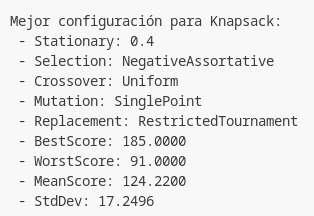
\includegraphics[width=0.45\linewidth]{img/r1.png}
	\label{fig:r1}
\end{figure}

Por otro lado, para un grafo con 50 ciudades mediante funciones de uniformidad generan el mejor resultado pero con una desviación estándar mucho mayor, lo que puede dificultar la búsqueda del óptimo global.

\begin{figure}[H]
	\centering
	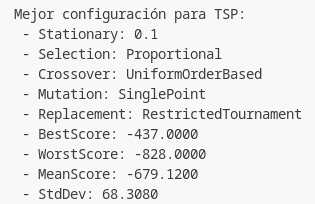
\includegraphics[width=0.45\linewidth]{img/r2}
	\label{fig:r2}
\end{figure}